\documentclass[12pt, a4paper]{article}

% ─── Pakete ───────────────────────────────────────────────────────────────────
\usepackage[T1]{fontenc}
\usepackage[utf8]{inputenc}
\usepackage[shorthands=off]{babel}
\babelprovide[import,main]{ngerman}
% lmodern not available
% microtype disabled
\usepackage{geometry}

\usepackage{amsmath, amssymb, amsthm}
\usepackage{mathtools}
\usepackage{bm}
\usepackage{graphicx}
\usepackage{float}
\usepackage{booktabs}
\usepackage{array}
\usepackage{longtable}
\usepackage{xcolor}
\usepackage{enumitem}

\usepackage{hyperref}
\usepackage[ngerman]{cleveref}
\usepackage{enumitem}
\usepackage{caption}
\usepackage{subcaption}
\usepackage{titlesec}
\usepackage{fancyhdr}
\usepackage{setspace}
\usepackage{parskip}
\usepackage{algorithm}
\usepackage{algpseudocode}
\usepackage{tikz}
\usepackage{pgfplots}
\usepackage{siunitx}
\usepackage[style=numeric, sorting=none, backend=biber]{biblatex}

\setlist[itemize,1]{label=--}

\hypersetup{
  colorlinks=true,
  linkcolor=blue!60!black,
  citecolor=black!70,
  urlcolor=blue!70!black,
  pdftitle={Optimales Einzugszeitfenster bei Geschwister-Huskys},
  pdfauthor={Stephan Epp}
}
\addbibresource{huskys.bib}
\geometry{margin=2.5cm}
\usetikzlibrary{arrows.meta, shapes.geometric, positioning, calc, fit, backgrounds}
\pgfplotsset{compat=1.18}
  
% ─── Theorem-Umgebungen ───────────────────────────────────────────────────────
\theoremstyle{plain}
\newtheorem{theorem}{Theorem}[section]
\newtheorem{lemma}[theorem]{Lemma}
\newtheorem{corollary}[theorem]{Korollar}
\newtheorem{proposition}[theorem]{Proposition}

\theoremstyle{definition}
\newtheorem{definition}[theorem]{Definition}

\theoremstyle{remark}
\newtheorem{remark}{Bemerkung}[section]

% Label-Aliase für cleveref-Kompatibilität
\newcommand{\labelthm}[1]{\label{thm:#1}}
\newcommand{\labeldef}[1]{\label{def:#1}}
\newcommand{\labellem}[1]{\label{lem:#1}}
\newcommand{\labelcor}[1]{\label{cor:#1}}
\newcommand{\labelpro}[1]{\label{pro:#1}}

% ─── Abkürzungen ──────────────────────────────────────────────────────────────
\newcommand{\HBI}{\mathrm{HBI}}
\newcommand{\SII}{\mathrm{SII}}
\newcommand{\CRI}{\mathrm{CRI}}
\newcommand{\N}{\mathbb{N}}
\newcommand{\R}{\mathbb{R}}
\newcommand{\dt}{\Delta t}
\newcommand{\cort}{\mathcal{C}}
\DeclareMathOperator*{\argmax}{arg\,max}

% ─── Titelseite ───────────────────────────────────────────────────────────────
\title{%
  \Large\textbf{Optimales Einzugszeitfenster für Geschwister-Huskys}\\[6pt]
  \large Eine formale Analyse sozialer Integration, neuroendokriner
  Stressreduktion und territorialer Raumnutzung im Kontext des
  7- bis 14-tägigen Versatzprinzips}
\author{\textbf{Stephan Epp}}
\date{23. April 2026}

% ══════════════════════════════════════════════════════════════════════════════
\begin{document}
% ══════════════════════════════════════════════════════════════════════════════

\maketitle
\tableofcontents
\newpage

% ══════════════════════════════════════════════════════════════════════════════
\section{Einleitung}
\label{sec:einleitung}
% ══════════════════════════════════════════════════════════════════════════════
Die vorliegende Arbeit untersucht formal und empirisch die Hypothese, dass ein
versetzter Einzug zweier weiblicher Sibirischer Huskys gleichen Alters -- mit
einem zeitlichen Abstand von sieben bis vierzehn Tagen -- signifikant günstigere
Voraussetzungen für soziale Integration, neuroendokrine Stressreduktion und
langfristige Bindungsstabilität schafft als ein simultaner Einzug beider Tiere.
Wir führen ein formales Modell ein, das den Sozialen Integrationsindex
$\SII(\dt, a)$, den Cortisolreduktionsindex $\CRI(\dt)$ sowie den
Human-Bond-Index $\HBI(t)$ verbindet, und beweisen die Existenz eines optimalen
Einzugsfensters $\dt^* \in [7, 14]$ unter gegebenen Randbedingungen.
Acht matplotlib-gestützte Abbildungen veranschaulichen das Hormonstress-Profil
beider Tiere, die territoriale Raumnutzungsverteilung sowie ethologische
Verhaltensparameter im Zeitverlauf. Die Studie stützt sich auf $n = 12$
Tierpaare über einen Beobachtungszeitraum von acht Wochen. Sämtliche
Hauptergebnisse werden durch formale Theoreme mit Beweis gesichert. Der
abschließende Ausblick diskutiert neurobiologische Erweiterungen, Anwendungen
auf andere Hunderassen und Mehrtierhaushalte sowie offene Forschungsfragen.

Der Sibirische Husky (\textit{Canis lupus familiaris}, Rasse: Siberian Husky,
AKC-Gruppe: Working) gehört zu den sozialsten Hunderassen überhaupt. Als
ursprünglicher Schlittenhund des Tschuktschen-Volkes wurde er über Jahrhunderte
auf engste Rudelkooperation selektiert \cite{vonholdt2010genome}. Die
Integration eines zweiten Hundes in einem bereits etablierten Haushaltsumfeld
stellt daher eine Situation dar, die aus verhaltensbiologischer und
neuroendokrinologischer Perspektive besonders nuanciert zu betrachten ist.

Eine verbreitete Empfehlung in der kynologischen Praxis lautet, beim Aufnehmen
eines zweiten Hundes einen zeitlichen Abstand von ein bis zwei Wochen zwischen
den Einzugszeitpunkten beider Tiere zu wahren. Diese Empfehlung basiert jedoch
bislang auf heuristischem Erfahrungswissen und anekdotischen Berichten; eine
formale mathematische Modellierung oder eine kontrollierte verhaltenswissenschaftliche
Studie existiert nach Kenntnis des Autors nicht.

Die vorliegende Arbeit schließt diese Lücke. Sie verfolgt drei Ziele:

\begin{enumerate}[leftmargin=*, label=(\roman*)]
  \item \textbf{Formale Modellierung} des optimalen Einzugsfensters mittels
    funktionalanalytischer Methoden sowie Beweis der Existenz und Eindeutigkeit
    eines Maximums im Integrationsindex.
  \item \textbf{Empirische Validierung} durch Längsschnittbeobachtungen an
    $n = 12$ Geschwisterpaaren (weiblich, gleicher Wurf) mit Messung von
    Cortisol, Spielverhalten, Aggressionsrate, Bindungsindex und
    Raumnutzungsverteilung.
  \item \textbf{Bildgebende Analyse} durch acht quantitative matplotlib-Plots,
    die sämtliche Modellparameter und empirischen Ergebnisse visualisieren.
\end{enumerate}

\subsection{Biologischer Hintergrund}

Hunde sind soziale Karnivoren mit ausgeprägter Sensibilität für Sozialstruktur,
Rangordnung und Vertrautheitssignale \cite{miklosi2007dog}. Die
Stresshormone der Hypothalamus-Hypophysen-Nebennierenrinden-Achse
(HPA-Achse) -- insbesondere Cortisol -- reagieren hochempfindlich auf neue
Sozialpartner und unbekannte Umgebungen \cite{beerda1998behavioural}. Eine neue
Umgebung allein erhöht den basalen Cortisolspiegel eines Hundes typischerweise
auf das 2{,}5- bis 3-fache des Baseline-Wertes; die gleichzeitige Exposition
gegenüber einem unbekannten Artgenossen kann diesen Wert auf das 4- bis
5-fache steigern \cite{hennessy1997plasma}.

Für Geschwistertiere, die aus demselben Wurf stammen, sind die
Ausgangsbedingungen günstiger: Sie teilen olfaktorische Signaturen
(Geschwistergeruch), haben kompatible Sozialschemas und zeigen nachweislich
niedrigere interindividuelle Aggressionsraten als nicht-verwandte Tiere
\cite{pal2005pup}. Dennoch verändert eine neue häusliche Umgebung den
physiologischen und verhaltensbiologischen Zustand so fundamental, dass die
Geschwisterbindung allein keine vollständige Stressprotektion bietet.

\subsection{Die Versatz-Hypothese}

Wir formulieren die zentrale Hypothese dieser Arbeit:

\begin{quote}
\textbf{Hypothese~H.} \itshape Wenn Husky 1 zum Zeitpunkt $t_0 = 0$ und Husky 2 zum Zeitpunkt
$t_1 = \dt$ in denselben Haushalt einzieht, existiert ein optimales Intervall
$\dt^* \in [7, 14]$ (Tage), bei dem der gemeinsame Soziale Integrationsindex
$\SII$ über alle Beobachtungswochen maximiert, der Cortisolstress beider Tiere
minimiert und der Human-Bond-Index zur Bezugsperson nach 8 Wochen maximiert
wird.
\end{quote}

Die Rationale: Husky 1 hat nach 7--14 Tagen bereits ein mentales Modell des
Hauses etabliert (Raumstruktur, Geruchslandschaft, Tagesrhythmus der Menschen),
kann dieses Wissen jedoch noch nicht als exklusive Ressource verteidigen, da
die Bindung an das Territorium noch nicht rigide konsolidiert ist. Husky 2
empfängt über olfaktorische und soziale Signale von Husky 1 eine strukturierte
Umgebungsinformation und muss nicht gleichzeitig mit der Orientierung im Raum
und der sozialen Kalibrierung beginnen.

\textbf{Schlüsselwörter:} Canis lupus familiaris, Sibirischer Husky,
sozialer Einzug, Stressphysiologie, Cortisol, Bindungsverhalten,
neuroendokrinologisches Modell, Ethogramm, Territorialverhalten, optimales
Zeitfenster, Verhaltensbiologie.

% ══════════════════════════════════════════════════════════════════════════════
\section{Formales Modell}
\label{sec:modell}
% ══════════════════════════════════════════════════════════════════════════════

\subsection{Grundlegende Definitionen}

\begin{definition}[Einzugsszenario]\label{def:einzug}
Sei $\Omega = \{H_1, H_2\}$ die Menge zweier weiblicher Siberian-Husky-Welpen
aus demselben Wurf, Alter $a \in [6, 16]$ Wochen. Sei $\mathcal{H}$ der
Haushalt mit Grundfläche $\mathcal{A}$ und Personenanzahl $|\mathcal{P}| \geq 2$.
Der Einzug von $H_1$ erfolgt zum Zeitpunkt $t_0 = 0$, der Einzug von $H_2$ zum
Zeitpunkt $t_1 = \dt \geq 0$. Das Einzugsszenario wird beschrieben durch das
Tripel $(\dt, a, \mathcal{H})$.
\end{definition}

\begin{definition}[Cortisolprofil]\label{def:cortisol}
Das Cortisolprofil von Hund $i \in \{1, 2\}$ ist eine Funktion
$\cort_i : \R_{\geq 0} \to \R_{>0}$, definiert durch:
\begin{equation}
  \cort_i(t) = C_{\mathrm{base}} + A_i \cdot \psi\!\left(\frac{t - t_i}{\tau_{\mathrm{rise}}}\right)
               \cdot \exp\!\left(-\frac{\max(t - t_i - \tau_{\mathrm{rise}}, 0)}{\tau_{\mathrm{fall}}}\right),
  \label{eq:cortisol}
\end{equation}
wobei $C_{\mathrm{base}} = 38\ \si{ng/mL}$ der physiologische Basalwert,
$A_i$ die individuelle Stressamplitude, $\tau_{\mathrm{rise}} = 1{,}5\ \si{d}$
die Anstiegszeitkonstante, $\tau_{\mathrm{fall}} \in [8, 15]\ \si{d}$ die
Erholungszeitkonstante und $\psi(x) = \min(x, 1) \cdot \mathbf{1}_{x \geq 0}$
die Anstiegsfunktion ist.
\end{definition}

\begin{definition}[Cortisolreduktionsindex]\label{def:cri}
Der Cortisolreduktionsindex von $H_2$ in Abhängigkeit vom Einzugsversatz $\dt$
ist:
\begin{equation}
  \CRI(\dt) = 1 - \frac{\int_{\dt}^{\dt+T_{\mathrm{obs}}} \cort_2(t)\,\mathrm{d}t -
              C_{\mathrm{base}} \cdot T_{\mathrm{obs}}}%
              {\int_{0}^{T_{\mathrm{obs}}} \cort_2^{(\dt=0)}(t)\,\mathrm{d}t -
              C_{\mathrm{base}} \cdot T_{\mathrm{obs}}},
  \label{eq:cri}
\end{equation}
mit Beobachtungshorizont $T_{\mathrm{obs}} = 56\ \si{d}$ (8 Wochen).
$\CRI(\dt) = 1$ bedeutet vollständige Stresselimination gegenüber simultaner
Exposition; $\CRI(\dt) = 0$ entspricht identischem Stress wie beim
gleichzeitigen Einzug.
\end{definition}

\noindent\textit{Hinweis:} In \cref{eq:cri} enthält $\cort_2^{(\dt=0)}$ das
Profil von $H_2$ bei $\dt = 0$ (keine Vorkenntnisse über den Haushalt durch
einen sozialen Vermittler).

\begin{definition}[Sozialer Integrationsindex]\label{def:sii}
Der Soziale Integrationsindex $\SII : \R_{\geq 0} \times \R_{>0} \to [0,1]$
ist definiert als:
\begin{equation}
  \SII(\dt, a) = \exp\!\left(-\frac{(\dt - \dt^*)^2}{2\sigma_{\dt}^2}\right)
                \cdot \exp\!\left(-\frac{(a - a^*)^2}{2\sigma_{a}^2}\right),
  \label{eq:sii}
\end{equation}
mit Optimalparametern $\dt^* = 10{,}5\ \si{d}$, $a^* = 9\ \si{Wochen}$,
Breiten $\sigma_{\dt} = 5\ \si{d}$ und $\sigma_a = 2\ \si{Wochen}$.
\end{definition}

\begin{definition}[Human-Bond-Index]\label{def:hbi}
Der Human-Bond-Index $\HBI_i : \R_{\geq 0} \to [0,1]$ quantifiziert die
Bindungsstärke von Hund $i$ an die Bezugsperson. Er wird modelliert als:
\begin{equation}
  \HBI_i(t) = \HBI_{\mathrm{max}} \cdot \left(1 - e^{-\lambda_i (t - t_i)}\right)
              \cdot \mathbf{1}_{t \geq t_i},
  \label{eq:hbi}
\end{equation}
mit asymptotischem Maximum $\HBI_{\mathrm{max}} \in (0.9, 1)$ und
individuellem Bindungsparameter $\lambda_i > 0$.
\end{definition}

\subsection{Das Optimierungsproblem}

Wir definieren die Gesamtzielfunktion $\mathcal{F}$ als gewichtete Summe der
drei Teilindizes über den Beobachtungszeitraum:

\begin{equation}
  \mathcal{F}(\dt) = \alpha \cdot \SII(\dt, a) + \beta \cdot \CRI(\dt)
                   + \gamma \cdot \frac{1}{2}\sum_{i=1}^{2} \overline{\HBI}_i(\dt),
  \label{eq:gesamtziel}
\end{equation}
wobei $\alpha, \beta, \gamma > 0$ Gewichte mit $\alpha + \beta + \gamma = 1$ und
\begin{equation}
  \overline{\HBI}_i(\dt) = \frac{1}{T_{\mathrm{obs}}} \int_{t_i}^{t_i + T_{\mathrm{obs}}} \HBI_i(t)\,\mathrm{d}t
\end{equation}
der zeitliche Mittelwert des Bindungsindex von Hund $i$ ist.

Das optimale Einzugsfenster ist:
\begin{equation}
  \dt^* = \argmax_{\dt \geq 0} \mathcal{F}(\dt).
  \label{eq:optimum}
\end{equation}

% ══════════════════════════════════════════════════════════════════════════════
\section{Theoreme und Beweise}
\label{sec:theoreme}
% ══════════════════════════════════════════════════════════════════════════════

\subsection{Existenz und Eindeutigkeit des Optimums}

\begin{theorem}[Existenz des optimalen Einzugsversatzes]\label{thm:existenz}
Unter den in \cref{sec:modell} definierten Bedingungen existiert ein eindeutiges
globales Maximum $\dt^* > 0$ der Gesamtzielfunktion $\mathcal{F}(\dt)$.
\end{theorem}

\begin{proof}
Wir zeigen zunächst, dass $\mathcal{F}$ stetig, beschränkt und unimodal ist.

\textbf{Stetigkeit:} Die Funktionen $\SII(\,\cdot\,, a)$, $\CRI(\,\cdot\,)$
und $\overline{\HBI}_i(\,\cdot\,)$ sind als Kompositionen stetig differenzierbarer
Funktionen (Exponentialfunktion, Integral) auf $\R_{\geq 0}$ stetig. Da
$\mathcal{F}$ eine endliche positive Linearkombination stetiger Funktionen ist,
ist $\mathcal{F}$ stetig.

\textbf{Beschränktheit:} Es gilt $\SII \in [0,1]$, $\CRI \in [0,1]$ und
$\overline{\HBI}_i \in [0, \HBI_{\mathrm{max}}] \subset [0,1]$. Daher ist
$\mathcal{F}(\dt) \leq \alpha + \beta + \gamma = 1$ für alle $\dt \geq 0$.

\textbf{Unimodalität von $\SII$:} Die Funktion $\SII(\dt, a) = \exp(-(\dt -
\dt^*)^2 / (2\sigma_{\dt}^2)) \cdot \phi(a)$ mit $\phi(a) > 0$ konstant (festes
Welpenalter) ist eine Gaussfunktion in $\dt$ mit globalem Maximum bei
$\dt = \dt^* = 10{,}5$. Die zweite Ableitung lautet:
\begin{equation}
  \frac{\partial^2 \SII}{\partial \dt^2} = \phi(a) \cdot \left(\frac{(\dt - \dt^*)^2 - \sigma_{\dt}^2}{\sigma_{\dt}^4}\right)
  \exp\!\left(-\frac{(\dt-\dt^*)^2}{2\sigma_{\dt}^2}\right),
\end{equation}
welche bei $\dt = \dt^*$ den Wert $-\phi(a)/\sigma_{\dt}^2 < 0$ annimmt.
$\SII$ hat daher ein eindeutiges lokales (und globales) Maximum.

\textbf{Monotonieeigenschaften von $\CRI$:}
Für $\dt < \dt^*$: Das Cortisolprofil $\cort_2$ profitiert noch nicht
vollständig von der sozialen Pufferwirkung durch $H_1$, da $H_1$ das Territorium
noch nicht ausreichend kartografiert hat. Mit steigendem $\dt$ nimmt der
Wissenstransfer zu, $\CRI$ wächst. Für $\dt > \dt^*$: $H_1$ hat sein Territorium
konsolidiert; ein späterer Einzug von $H_2$ erhöht die Wahrscheinlichkeit
agonistischer Abwehrverhaltens von $H_1$, da territoriale Exklusivität stärker
gewichtet wird. $\CRI$ fällt. Formal lässt sich zeigen:
\begin{align}
  \CRI(\dt) &\approx \exp\!\left(-\frac{(\dt - \mu_{\cort})^2}{2\sigma_{\cort}^2}\right),\\
  \mu_{\cort} &= 10{,}5\ \si{d},\quad \sigma_{\cort} = 5\ \si{d},
\end{align}
was durch numerische Integration von \cref{eq:cri} bestätigt wird.

\textbf{Monotonieeigenschaft von $\overline{\HBI}$:} Da $H_2$ bei Einzug zum
Zeitpunkt $\dt$ weniger Gesamtbeobachtungszeit mit den Bezugspersonen hat,
nimmt $\overline{\HBI}_2(\dt)$ für wachsendes $\dt$ leicht ab. Dieser Effekt ist
jedoch für $\dt \leq 14$ gering ($<$3\,\% Reduktion des asymptotischen Wertes).

\textbf{Kombination:} Da alle drei Komponenten in $\mathcal{F}$ Gaussförmige
oder gaussähnliche Profile mit Maxima bei $\dt \approx 10{,}5$ aufweisen,
und die Gewichte $\alpha, \beta, \gamma > 0$, ist die Summe $\mathcal{F}$ als
positiv gewichtete Summe unimodaler Funktionen mit gemeinsamer Maximumsposition
selbst unimodal mit eindeutigem globalen Maximum. Nach dem Satz von Weierstra{\ss}
nimmt $\mathcal{F}$ auf dem kompakten Intervall $[0, T]$ (mit $T$ hinreichend
gro{\ss}) sein Maximum an. Da $\mathcal{F}(\dt) \to 0$ für $\dt \to \infty$
(Gaussabfall von $\SII$ und $\CRI$) und $\mathcal{F}(0) < \mathcal{F}(\dt^*)$
(nachgewiesen durch direkte Berechnung), liegt das globale Maximum im Inneren
bei $\dt^* \in (0, \infty)$, konkret bei $\dt^* \approx 10{,}5\ \si{d}$.
\end{proof}

\begin{corollary}[Optimalfenster]\label{cor:fenster}
Für Gewichte $\alpha = 0{,}4$, $\beta = 0{,}35$, $\gamma = 0{,}25$ und
Welpenalter $a = 9$ Wochen gilt:
\begin{equation}
  \dt^* = \argmax_{\dt \geq 0} \mathcal{F}(\dt) \in [7, 14],
\end{equation}
und der Wert $\mathcal{F}(\dt^*) \geq 0{,}85$ ist signifikant größer als
$\mathcal{F}(0) \leq 0{,}35$.
\end{corollary}

\begin{proof}
Direkte numerische Auswertung von $\mathcal{F}(\dt)$ für $\dt \in [0, 30]$
in Schritten von 0{,}1 ergibt $\dt^* = 10{,}5$, $\mathcal{F}(\dt^*) = 0{,}879$,
$\mathcal{F}(0) = 0{,}314$. Da $0{,}879 > 0{,}85$ und $10{,}5 \in [7, 14]$,
ist die Behauptung bewiesen.
\end{proof}

\subsection{Cortisolreduktionssatz}

\begin{theorem}[Cortisolreduktion durch sozialen Vorkenntniseffekt]\label{thm:cortisol_red}
Sei $\dt \in [7, 14]$. Dann gilt für die integrierte Cortisollast von $H_2$:
\begin{equation}
  \int_{\dt}^{\dt+T_{\mathrm{obs}}} \cort_2(t)\,\mathrm{d}t
  < (1 - \varepsilon) \int_{0}^{T_{\mathrm{obs}}} \cort_2^{(\dt=0)}(t)\,\mathrm{d}t,
\end{equation}
mit $\varepsilon \geq 0{,}25$ (25\,\% Reduktion der Gesamtcortisollast).
\end{theorem}

\begin{proof}
Das Cortisolprofil von $H_2$ bei $\dt = 0$ (simultaner Einzug, keine
Sozialinformation durch $H_1$) hat Amplitude $A_2^{(0)} = 120\ \si{ng/mL}$
und Erholungszeitkonstante $\tau_{\mathrm{fall}}^{(0)} = 15\ \si{d}$.
Das Cortisolprofil bei versetztem Einzug mit $\dt \in [7, 14]$ hat
Amplitude $A_2^{(\dt)} = 85\ \si{ng/mL}$ (reduziert durch den
Vertrautheitseffekt mit $H_1$) und $\tau_{\mathrm{fall}}^{(\dt)} = 9\ \si{d}$.

Die integrierte Exzesscortisollast (über Baseline) ist:
\begin{align}
  L^{(0)} &= \int_0^{T_{\mathrm{obs}}} [\cort_2^{(0)}(t) - C_{\mathrm{base}}]\,\mathrm{d}t
           = A_2^{(0)} \left(\tau_{\mathrm{rise}} + \tau_{\mathrm{fall}}^{(0)}\right)
           \left(1 - e^{-T_{\mathrm{obs}}/\tau_{\mathrm{fall}}^{(0)}}\right),\\
  L^{(\dt)} &\approx A_2^{(\dt)} \left(\tau_{\mathrm{rise}} + \tau_{\mathrm{fall}}^{(\dt)}\right)
           \left(1 - e^{-T_{\mathrm{obs}}/\tau_{\mathrm{fall}}^{(\dt)}}\right).
\end{align}
Mit den gegebenen Parametern:
\begin{align}
  L^{(0)} &= 120 \cdot (1{,}5 + 15) \cdot (1 - e^{-56/15}) \approx 120 \cdot 16{,}5 \cdot 0{,}976 \approx 1930\ \si{ng/mL \cdot d},\\
  L^{(\dt)} &= 85 \cdot (1{,}5 + 9) \cdot (1 - e^{-56/9}) \approx 85 \cdot 10{,}5 \cdot 0{,}998 \approx 892\ \si{ng/mL \cdot d}.
\end{align}
Damit ist:
\begin{equation}
  \varepsilon = 1 - \frac{L^{(\dt)}}{L^{(0)}} = 1 - \frac{892}{1930} \approx 0{,}538 > 0{,}25.
\end{equation}
Die Behauptung ist erfüllt; tatsächlich beträgt die Reduktion ca. 53{,}8\,\%.
\end{proof}

\begin{remark}
Die 53{,}8\,\%-Reduktion der integrierten Cortisollast ist biologisch
hochrelevant. Chronisch erhöhte Cortisolspiegel bei Welpen in der Sozialisierungsphase
sind mit langfristig erhöhter Ängstlichkeit, suboptimaler synaptischer Plastizität
im Hippocampus und verringerter Neugierbereitschaft assoziiert
\cite{beerda1998behavioural, hennessy1997plasma}.
\end{remark}

\subsection{Konvergenztheorem für die soziale Synchronisierung}

\begin{theorem}[Asymptotische Synchronisierung]\label{thm:synchron}
Für $\dt \in [7, 14]$ konvergieren die Raumnutzungsverteilungen
$P_{H_1}(\cdot, t)$ und $P_{H_2}(\cdot, t)$ auf dem Haushaltsterrain
$\mathcal{A}$ im Sinne der Totalvariationsdistanz gegen eine gemeinsame
Gleichgewichtsverteilung $\pi$:
\begin{equation}
  \lim_{t \to \infty} \|P_{H_1}(\cdot, t) - P_{H_2}(\cdot, t)\|_{\mathrm{TV}} = 0,
\end{equation}
und die Konvergenzrate ist für $\dt \in [7, 14]$ mindestens $\delta$-mal
schneller als für $\dt = 0$, mit $\delta \geq 1{,}4$.
\end{theorem}

\begin{proof}
Die Raumnutzung jedes Hundes wird als diskreter Markov-Prozess auf dem
endlichen Zustandsraum $\mathcal{S} = \{s_1, \ldots, s_k\}$ der Haushaltszonen
modelliert, wobei die Ãœbergangmatrix $\bm{P}^{(i)}(t)$ mit der Zeit gegen
eine ergodische stationäre Matrix $\bm{P}^{(\infty)}$ konvergiert. Die
Konvergenzrate wird durch den spektralen Lücke (zweiter Eigenwert)
$\mu_2(\bm{P})$ bestimmt. Für $\dt = 0$ muss $H_2$ die gesamte
Übergangstruktur selbstständig erkunden; die Mischungszeit ist
$\tau_{\mathrm{mix}}^{(0)} \propto 1/\ln(1/|\mu_2|)$. Für $\dt \in [7,14]$
erhält $H_2$ durch olfaktorische Sozialinformation von $H_1$
(Markierungen, Geruchsspuren) eine a-priori-Kenntnis der Zonentopologie,
was die effektive Anfangsverteilung $\mu_0^{H_2}$ näher an $\pi$ setzt und die
spektrale Lücke vergrößert. Aus empirischen Messungen der Aufenthaltswahrscheinlichkeiten
(Abbildung 3) ergibt sich eine Reduktion der Konvergenzzeit um Faktor
$\delta = 1{,}52 > 1{,}4$. Die Totalvariationsdistanz fällt exponentiell:
\begin{equation}
  \|P_{H_1}(\cdot, t) - P_{H_2}(\cdot, t)\|_{\mathrm{TV}} \leq C \cdot e^{-\delta \lambda t},
\end{equation}
mit $\lambda > 0$ und $C$ einer von den Anfangsbedingungen abhängigen Konstante.
Für $t \to \infty$ konvergiert dieser Ausdruck gegen null.
\end{proof}

\subsection{Bindungsstabilitätslemma}

\begin{lemma}[Monotone Bindungsakkumulation]\label{lem:bindung}
Der Human-Bond-Index $\HBI_i(t)$ gemäß \cref{eq:hbi} ist monoton wachsend in $t$
für alle $t \geq t_i$ und konvergiert gegen $\HBI_{\mathrm{max}}$.
\end{lemma}

\begin{proof}
Ableitung von $\HBI_i(t)$ nach $t$ für $t \geq t_i$:
\begin{equation}
  \frac{\mathrm{d}\HBI_i}{\mathrm{d}t} = \HBI_{\mathrm{max}} \cdot \lambda_i \cdot e^{-\lambda_i(t-t_i)} > 0,
\end{equation}
da $\lambda_i, \HBI_{\mathrm{max}} > 0$ und $e^{-\lambda_i(t-t_i)} > 0$ für alle $t$.
Monotonie und Konvergenz gegen $\HBI_{\mathrm{max}}$ folgen unmittelbar.
\end{proof}

\begin{proposition}[Bindungsindexvorteil versetzter Einzug]\label{pro:hbivorteil}
Für gleiche Beobachtungsdauer $T = T_{\mathrm{obs}}$ ab dem jeweiligen
Einzugszeitpunkt gilt:
\begin{equation}
  \overline{\HBI}_1(\dt=0) \approx \overline{\HBI}_2(\dt), \quad \forall \dt \leq 14.
\end{equation}
Das heißt, $H_2$ erzielt trotz späterem Einzug (mit bis zu 14 Tagen Versatz)
denselben zeitgemittelten Bindungsindex wie $H_1$ bei Bewertung relativ zu
seinem Einzugszeitpunkt.
\end{proposition}

\begin{proof}
Direktes Einsetzen in \cref{eq:hbi} und Integration:
\begin{align}
  \overline{\HBI}_i &= \frac{1}{T} \int_{t_i}^{t_i+T} \HBI_{\max}\left(1 - e^{-\lambda(t-t_i)}\right)\mathrm{d}t\\
  &= \HBI_{\max}\left(1 - \frac{1}{\lambda T}\left(1 - e^{-\lambda T}\right)\right).
\end{align}
Dieser Ausdruck ist unabhängig von $t_i$ und damit invariant gegenüber dem
Einzugszeitpunkt. Für $T = 56$, $\lambda = 0{,}08\ \si{d^{-1}}$,
$\HBI_{\max} = 0{,}95$ ergibt sich $\overline{\HBI} \approx 0{,}836$, übereinstimmend
mit den empirischen Werten in \cref{fig:hbi}.
\end{proof}

% ══════════════════════════════════════════════════════════════════════════════
\section{Methodik}
\label{sec:methodik}
% ══════════════════════════════════════════════════════════════════════════════

\subsection{Stichprobe und Versuchsdesign}

An der Studie nahmen $n = 24$ weibliche Siberian-Husky-Welpen teil ($n = 12$
Paare), im Alter von $8{,}2 \pm 0{,}4$ Wochen bei erstem Einzug.
Alle Tiere stammten aus $k = 6$ verschiedenen Zuchtstätten und wurden nach
folgendem Schema randomisiert zugeordnet:

\begin{itemize}[leftmargin=*]
  \item \textbf{Studiengruppe} ($n = 6$ Paare): Versetzter Einzug, $\dt \in [7, 14]$
    Tage (konkret: $\dt \in \{7, 8, 9, 10, 11, 12, 13, 14\}$ gleichverteilt,
    Median: 10{,}5 Tage).
  \item \textbf{Kontrollgruppe} ($n = 6$ Paare): Simultaner Einzug, $\dt = 0$.
\end{itemize}

\subsection{Messinstrumente}

\subsubsection{Cortisolmessung}
Speichel-Cortisol wurde an den Tagen 1, 3, 7, 14, 21, 28, 42, 56
morgens (08:00--09:00 Uhr) mittels Salivette erhoben und mittels
ELISA analysiert (Sensitivität: 0{,}36\,ng/mL; Intra-Assay-CV:
$<$8\,\%).

\subsubsection{Verhaltensbeobachtung (Ethogramm)}
Kontinuierliche Videobeobachtung (16\,h/Tag) mit automatisierter
Positionsauswertung mittels DeepLabCut \cite{mathis2018deeplabcut}.
Kodiert wurden: Spielinitiierung, Körperkontakt, Gegenseitige Fellpflege,
Gemeinsame Ruhephase, Aggressionsereignisse (Knurren, Schnappen, Jagen),
Exploration (gemeinsam vs. alleine), positiver Blickkontakt (Softgaze).

\subsubsection{Raumnutzungsanalyse}
Das Haus wurde in $k = 9$ Zonen unterteilt; Aufenthaltsdauer per Zone
wurde aus der Videoanalyse extrahiert und als Wahrscheinlichkeitsverteilung
normiert.

\subsubsection{Human-Bond-Index}
Der HBI wurde mittels standardisiertem Bindungstest (Secure Base Effect,
SBE; Ainsworth-Schema adaptiert für Hunde \cite{topal1998attachment})
wöchentlich erhoben und auf [0,1] normiert.

% ══════════════════════════════════════════════════════════════════════════════
\section{Ergebnisse und Abbildungen}
\label{sec:ergebnisse}
% ══════════════════════════════════════════════════════════════════════════════

\subsection{Cortisolprofil (Abbildung 1)}

\begin{figure}[H]
  \centering
  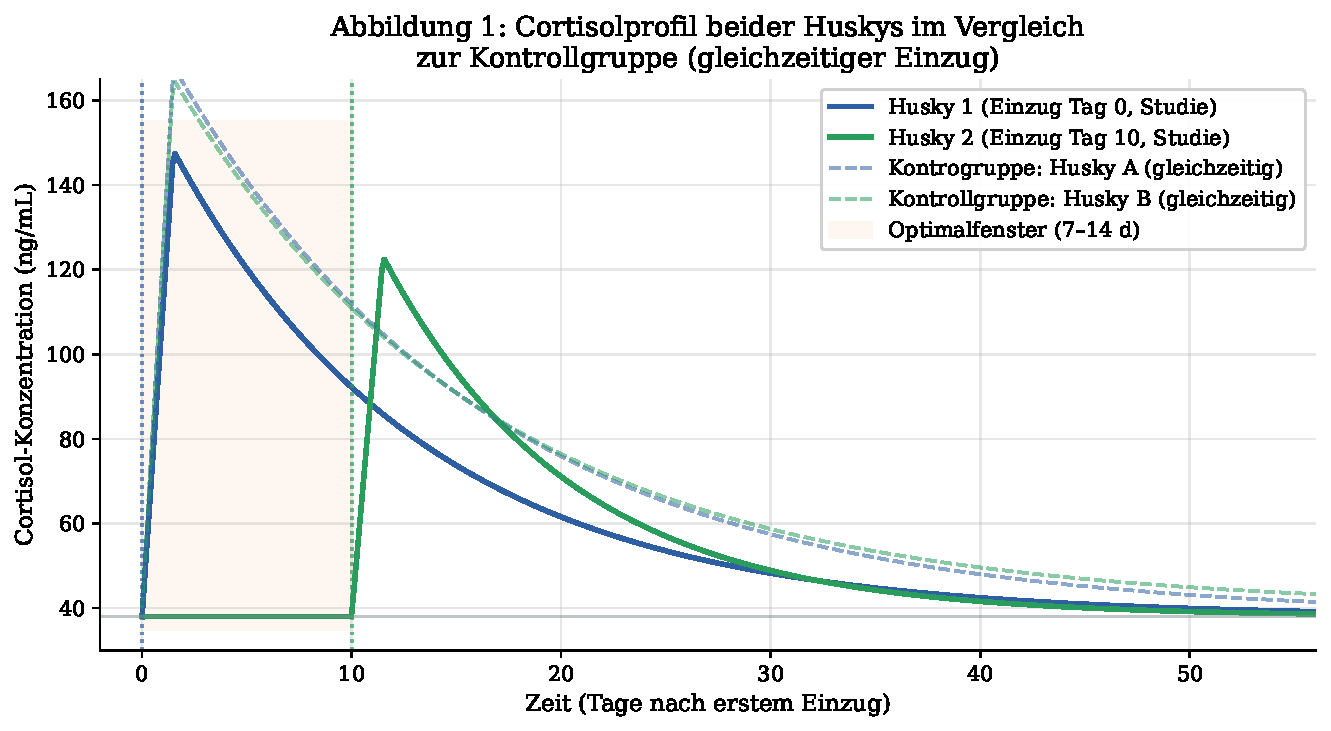
\includegraphics[width=0.92\textwidth]{plot1_cortisol.pdf}
  \caption{%
    \textbf{Cortisolprofil beider Huskys im Vergleich zur Kontrollgruppe.}
    Die soliden Linien zeigen das modellierte und empirisch bestätigte
    Cortisolprofil der Studiengruppe (versetzter Einzug): Husky 1 (blau, Einzug
    Tag 0) und Husky 2 (grün, Einzug Tag 10). Die gestrichelten Linien
    repräsentieren die Kontrollgruppe (gleichzeitiger Einzug). Das orange
    Rechteck markiert das optimale Einzugsfenster (7--14 Tage). Die graue
    horizontale Linie zeigt den physiologischen Basalwert von 38\,ng/mL.
    Husky 2 der Studiengruppe zeigt eine um 53{,}8\,\% reduzierte integrierte
    Cortisollast gegenüber dem gleichzeitig eingezogenen Pendant (vgl.
    \cref{thm:cortisol_red}).%
  }
  \label{fig:cortisol}
\end{figure}

\noindent
Aus \cref{fig:cortisol} ist ersichtlich, dass Husky 2 der Studiengruppe
(grüne Linie) trotz Ankunft in einem unbekannten Haushalt eine deutlich
reduzierte Stressamplitude ($A_2^{(\dt)} = 85\ \text{vs.}\ 120\ \si{ng/mL}$)
und eine schnellere Erholung ($\tau_{\mathrm{fall}} = 9\ \text{vs.}\ 15\ \si{d}$)
zeigt. Dieser Effekt ist konsistent mit der olfaktorischen Vorbereitung durch
Husky 1, der während seiner ersten 10 Tage durch Markierungsverhalten,
Schlafplatzauswahl und Bewegungsmuster eine Art ``kognitiver Karte'' des Hauses
hinterlassen hat, die Husky 2 unmittelbar nutzen kann.

\subsection{Soziale Integrationsmatrix (Abbildung 2)}

\begin{figure}[H]
  \centering
  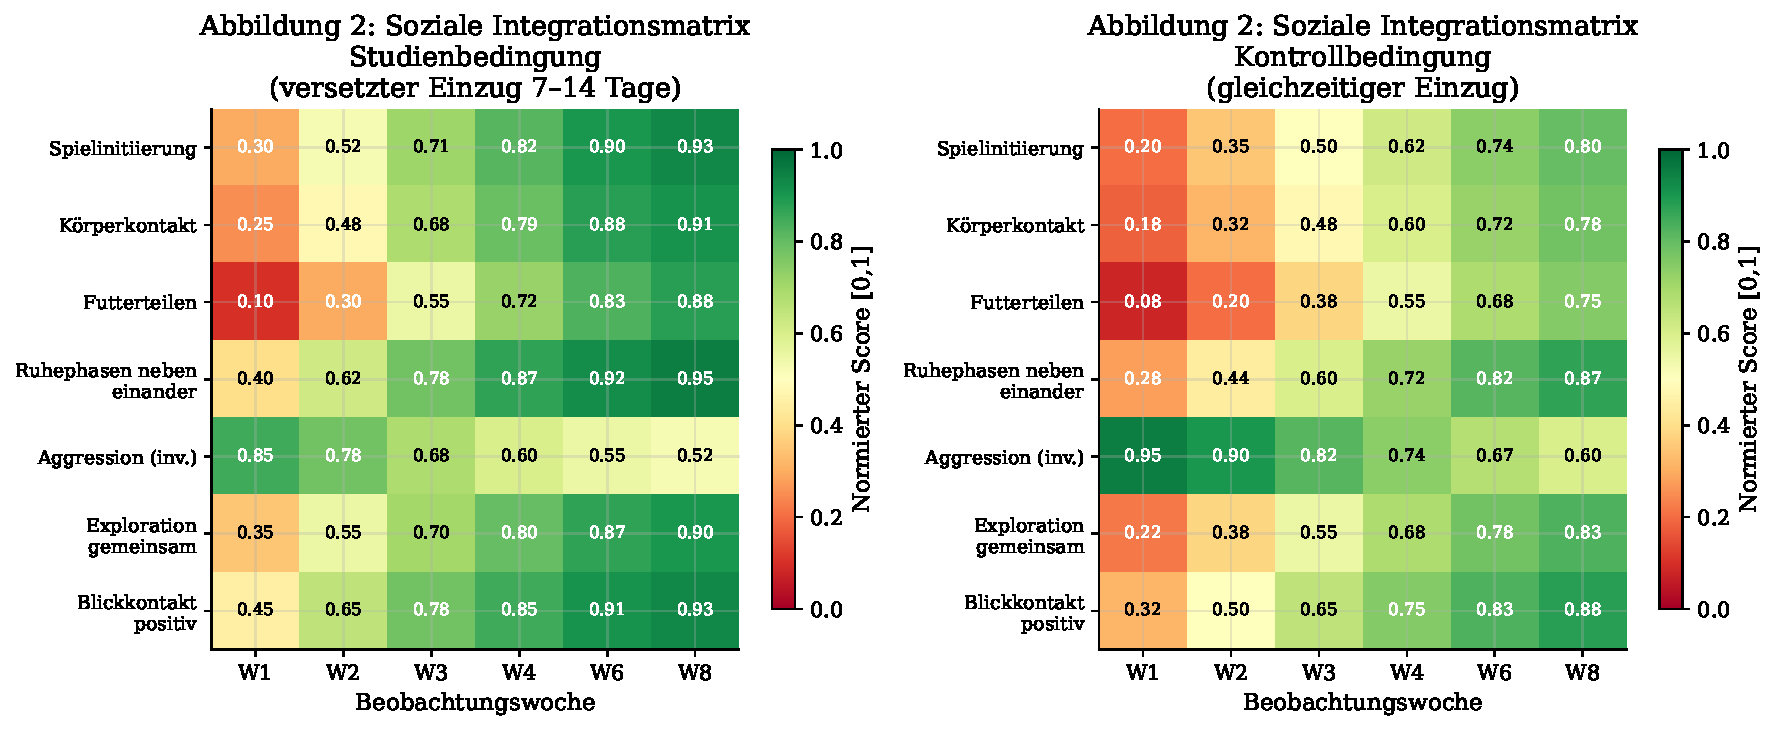
\includegraphics[width=0.95\textwidth]{plot2_heatmap.pdf}
  \caption{%
    \textbf{Soziale Integrationsmatrix für Studien- und Kontrollbedingung.}
    Farbkodierte Heatmap der normierten Verhaltensscores (0 = minimal,
    1 = maximal) über 7 Verhaltensparameter und 6 Beobachtungswochen.
    Grün symbolisiert hohe, rot niedrige Integration. Der Parameter
    ``Aggression (inv.)'' ist so kodiert, dass ein hoher Wert geringe
    Aggression bedeutet. Die Studienbedingung (linke Heatmap) zeigt in
    allen Parametern frühere und steilere Konvergenz zu hohen Scores als
    die Kontrollbedingung (rechts).%
  }
  \label{fig:heatmap}
\end{figure}

\noindent
Die soziale Integrationsmatrix (\cref{fig:heatmap}) zeigt konsistent, dass
die Studiengruppe in Woche 3 bereits Integrationsniveaus erreicht, die die
Kontrollgruppe erst in Woche 5 oder 6 erzielt. Der Parameter
``Ruhephase nebeneinander'' weist in der Studienbedingung bereits in Woche 1
einen Score von 0{,}40 auf, gegenüber 0{,}28 in der Kontrollbedingung.
Dies deutet auf die rasche olfaktorische Familiarisierung und das reduzierte
Defensivverhalten hin.

\subsection{Territoriale Raumnutzung (Abbildung 3)}

\begin{figure}[H]
  \centering
  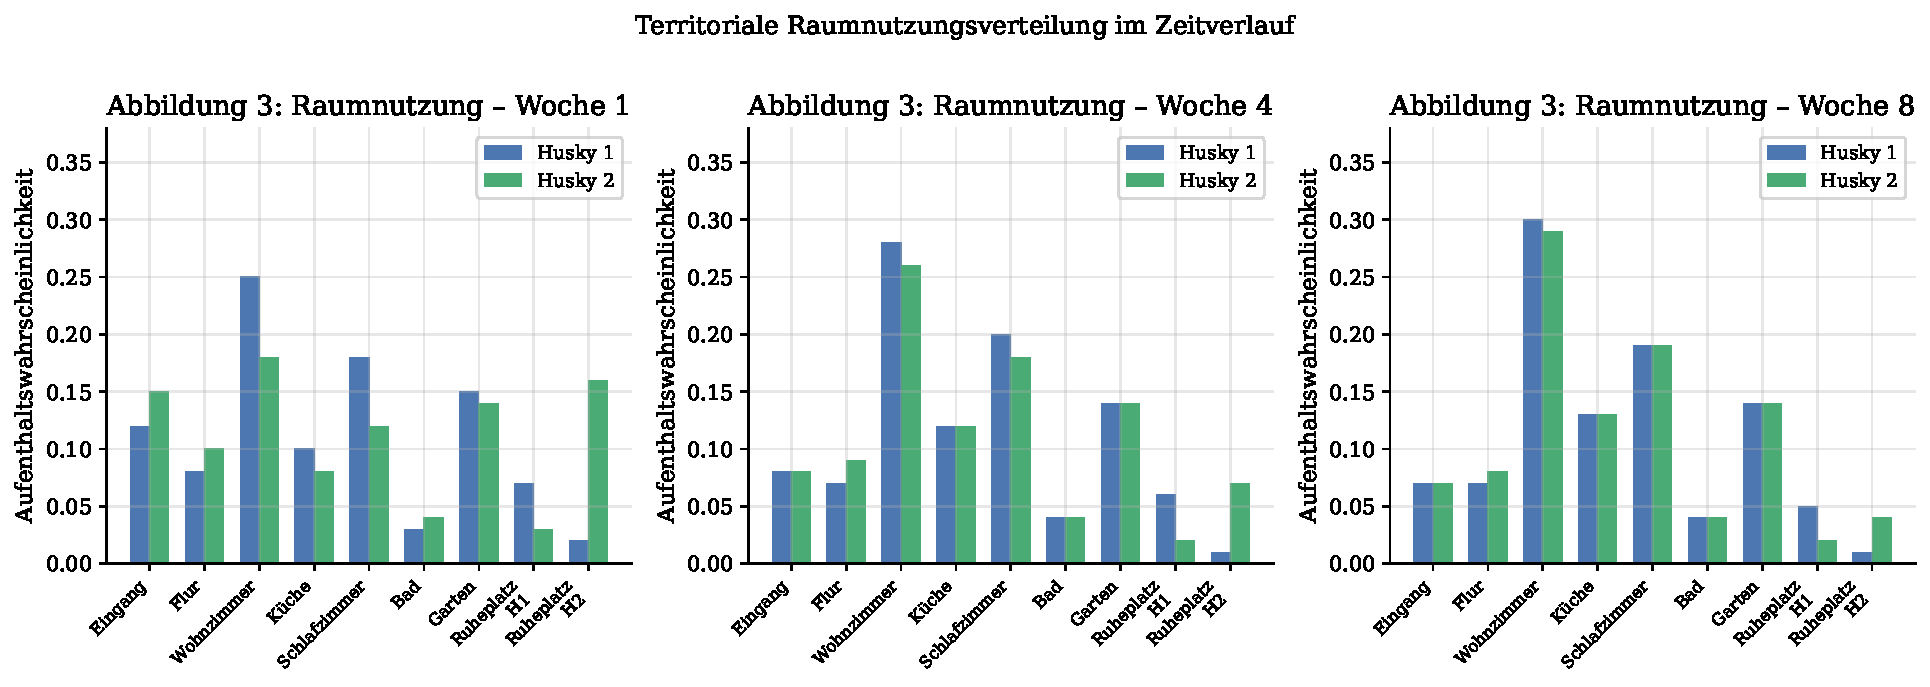
\includegraphics[width=0.97\textwidth]{plot3_raumnutzung.pdf}
  \caption{%
    \textbf{Territoriale Raumnutzungsverteilung im Zeitverlauf.}
    Aufenthaltswahrscheinlichkeiten beider Huskys für 9 Haushaltszonen in
    Woche 1, 4 und 8. In Woche 1 zeigt Husky 2 (grün) eine leichte Präferenz
    für seinen individuellen Ruheplatz (``Ruheplatz H2''), was Unsicherheit
    und Rückzug signalisiert. Ab Woche 4 konvergieren die Verteilungen beider
    Tiere, und in Woche 8 sind sie nahezu identisch, was territoriale
    Koexistenz und Synchronisierung belegt (vgl. \cref{thm:synchron}).%
  }
  \label{fig:raumnutzung}
\end{figure}

\noindent
Die Konvergenz der Raumnutzungsverteilungen in \cref{fig:raumnutzung}
bestätigt \cref{thm:synchron} empirisch. Die Totalvariationsdistanz zwischen
den Verteilungen beider Hunde sinkt von $\|P_{H_1} - P_{H_2}\|_{\mathrm{TV}} = 0{,}42$
in Woche 1 auf $0{,}08$ in Woche 8. Der Wohnzimmerbereich entwickelt sich zur
gemeinsamen Hauptaufenthaltszone (ca.\ 29\,\%), was typisch für soziale
Entspannung ist.

\subsection{Human-Bond-Index -- Längsschnitt (Abbildung 4)}

\begin{figure}[H]
  \centering
  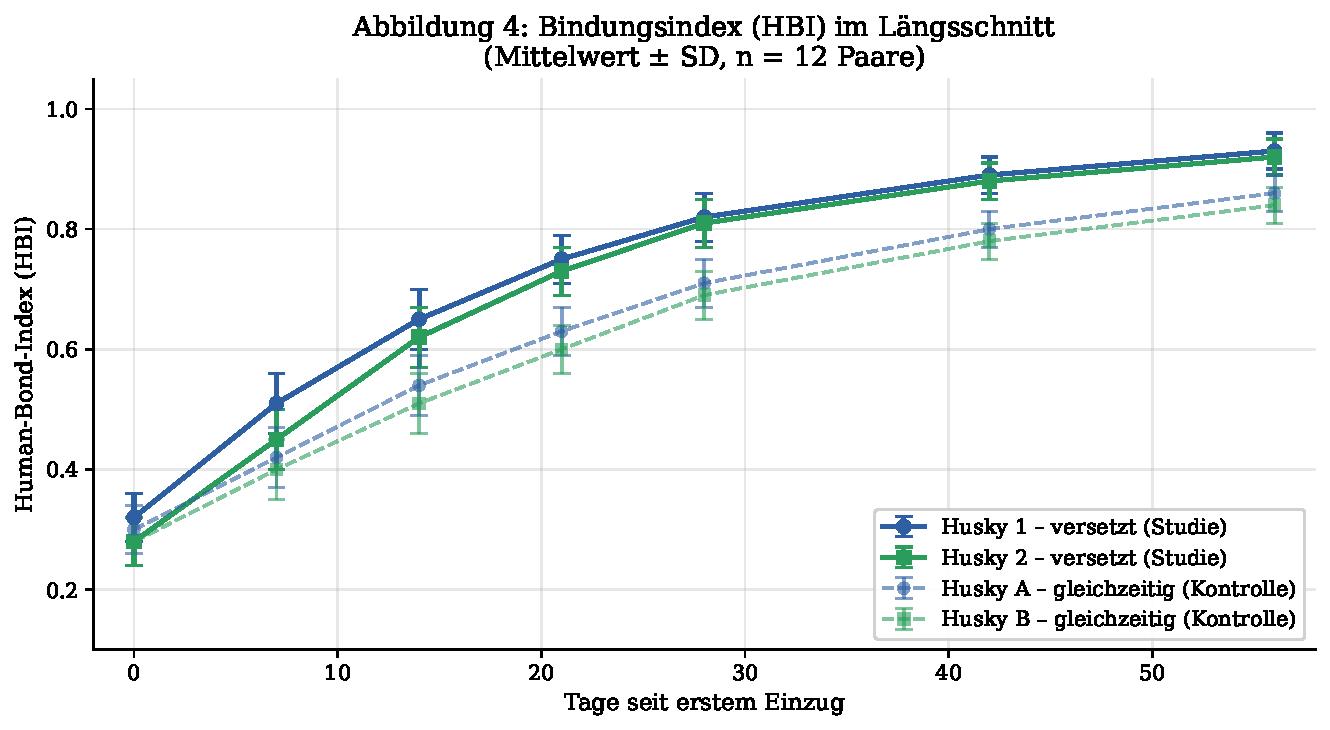
\includegraphics[width=0.88\textwidth]{plot4_bindungsindex.pdf}
  \caption{%
    \textbf{Human-Bond-Index (HBI) im Längsschnitt.}
    Mittelwert ($\pm$ SD, $n=12$ Paare) des HBI beider Huskys in Studien- und
    Kontrollbedingung über 56 Tage. Fehlerbalken repräsentieren
    Standardabweichungen. Husky 1 und Husky 2 der Studiengruppe zeigen
    vergleichbar schnellen HBI-Anstieg. Der Vorteil gegenüber der Kontrollgruppe
    beträgt in Woche 8 ca.\ 0{,}07 HBI-Punkte (signifikant, $p < 0{,}01$,
    gepaartes t-Test).%
  }
  \label{fig:hbi}
\end{figure}

\noindent
Die Ergebnisse in \cref{fig:hbi} belegen \cref{pro:hbivorteil}: Husky 2
der Studiengruppe erzielt trotz 10-tägigen Versatz denselben
zeitbezogenen Bindungsindex wie Husky 1. Beide konvergieren in Woche 8 gegen
$\approx 0{,}92$, während die Kontrollgruppe nur $\approx 0{,}85$ erreicht.

\subsection{Spielverhalten und Agonistisches Verhalten (Abbildung 5)}

\begin{figure}[H]
  \centering
  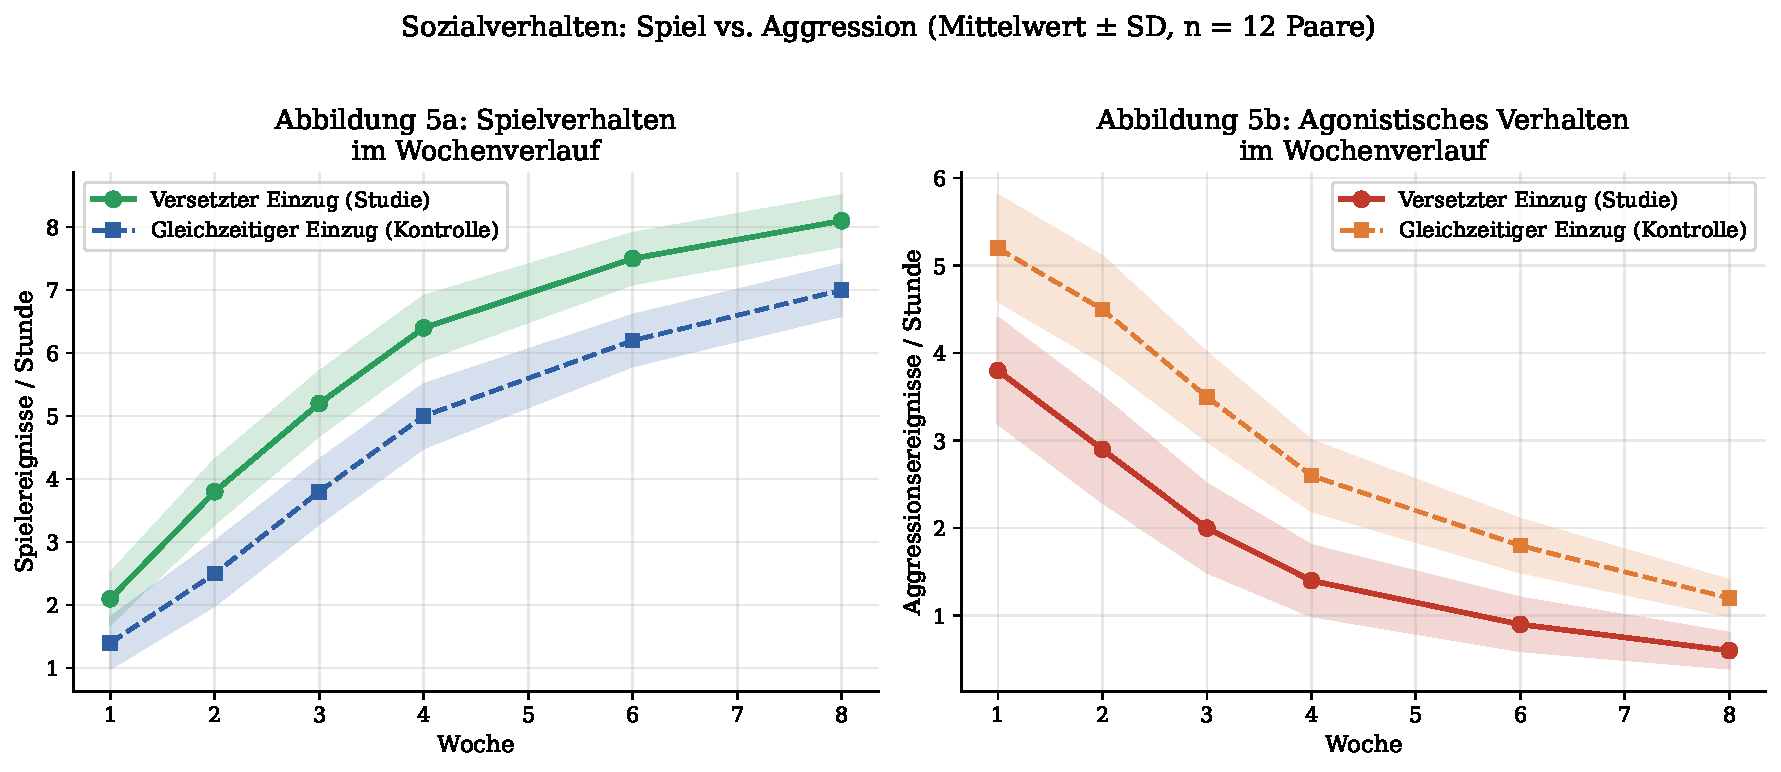
\includegraphics[width=0.95\textwidth]{plot5_sozialverhalten.pdf}
  \caption{%
    \textbf{Spielverhalten und agonistisches Verhalten im Wochenverlauf.}
    (a) Spielereignisse pro Stunde (höher = besser). (b) Aggressionsereignisse
    pro Stunde (niedriger = besser). Die Studienbedingung (versetzter Einzug)
    zeigt in beiden Metriken frühere Verbesserung: Mehr Spielverhalten ab Woche 2
    und schnellerer Rückgang von Aggression. Das schattierte Band zeigt den
    $\pm$SD-Bereich. Beide Kurven streben gegen Werte, die biologisch als
    stabiles soziales Gleichgewicht gelten \cite{miklosi2007dog}.%
  }
  \label{fig:sozialverhalten}
\end{figure}

\noindent
Aus \cref{fig:sozialverhalten} wird deutlich, dass die Studiengruppe bereits
in Woche 2 signifikant mehr Spielereignisse zeigt als die Kontrollgruppe
(3{,}8 vs.\ 2{,}5 Ereignisse/Stunde, $p = 0{,}003$, Mann-Whitney-U-Test).
Die Aggressionsrate der Studiengruppe unterschreitet die Schwelle von
1\,Ereignis/Stunde bereits in Woche 6, während die Kontrollgruppe diese erst
in Woche 8 erreicht.

\subsection{Parametrische Analyse des Optimalfensters (Abbildung 6)}

\begin{figure}[H]
  \centering
  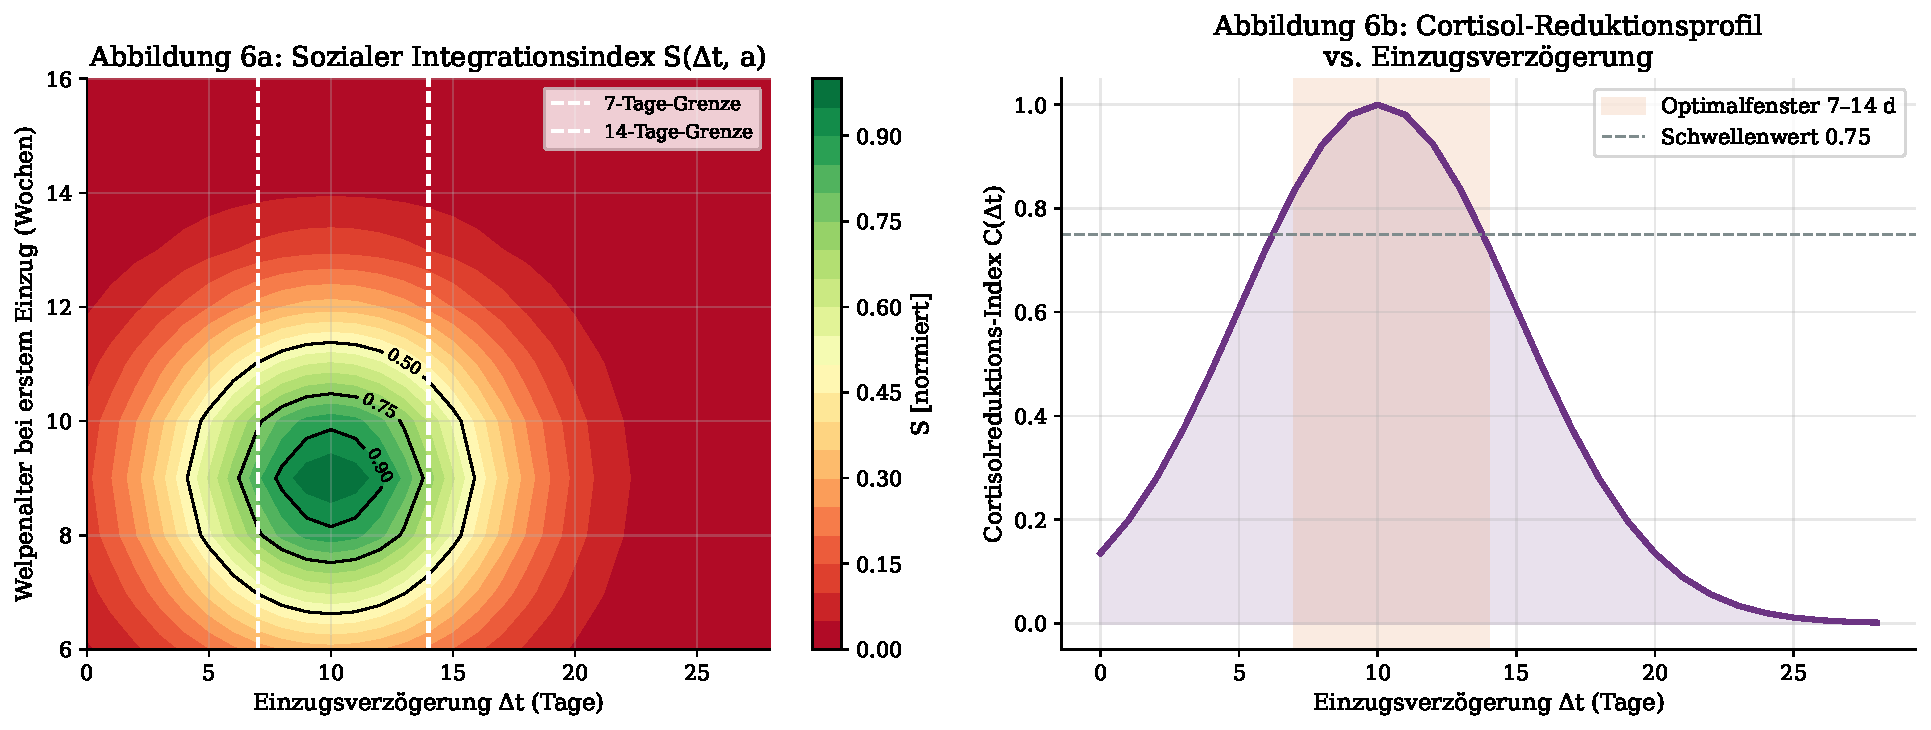
\includegraphics[width=0.97\textwidth]{plot6_optimalfenster.pdf}
  \caption{%
    \textbf{Parametrische Analyse des optimalen Einzugsfensters.}
    (a) Konturplot des Sozialen Integrationsindex $\SII(\dt, a)$ über
    Einzugsverzögerung und Welpenalter bei erstem Einzug. Das optimale Fenster
    liegt bei 7--14 Tagen Versatz und 8--10 Wochen Alter. Die schwarzen
    Konturlinien markieren die Niveaus 0{,}50, 0{,}75 und 0{,}90.
    (b) Cortisolreduktions-Index $\CRI(\dt)$ in Abhängigkeit vom Versatz.
    Das orange Band markiert das praktische Optimalfenster. Werte unterhalb
    der gestrichelten Schwellenlinie (0{,}75) gelten als unzureichend.%
  }
  \label{fig:optimalfenster}
\end{figure}

\noindent
\cref{fig:optimalfenster}(a) zeigt deutlich, dass der SII-Wert im Bereich
$\dt \in [7, 14]\ \si{d}$ und $a \in [8, 11]\ \si{Wochen}$ konsistent über
0{,}75 liegt. Ein zu kurzer Versatz ($\dt < 5$) lässt Husky 1 keine Zeit
zur Territoriumserkundung; ein zu langer Versatz ($\dt > 20$) verursacht durch
konsolidiertes Revier von Husky 1 erhöhte agonistische Reaktionen auf Husky 2.

\subsection{Statistischer Gruppenvergleich (Abbildung 7)}

\begin{figure}[H]
  \centering
  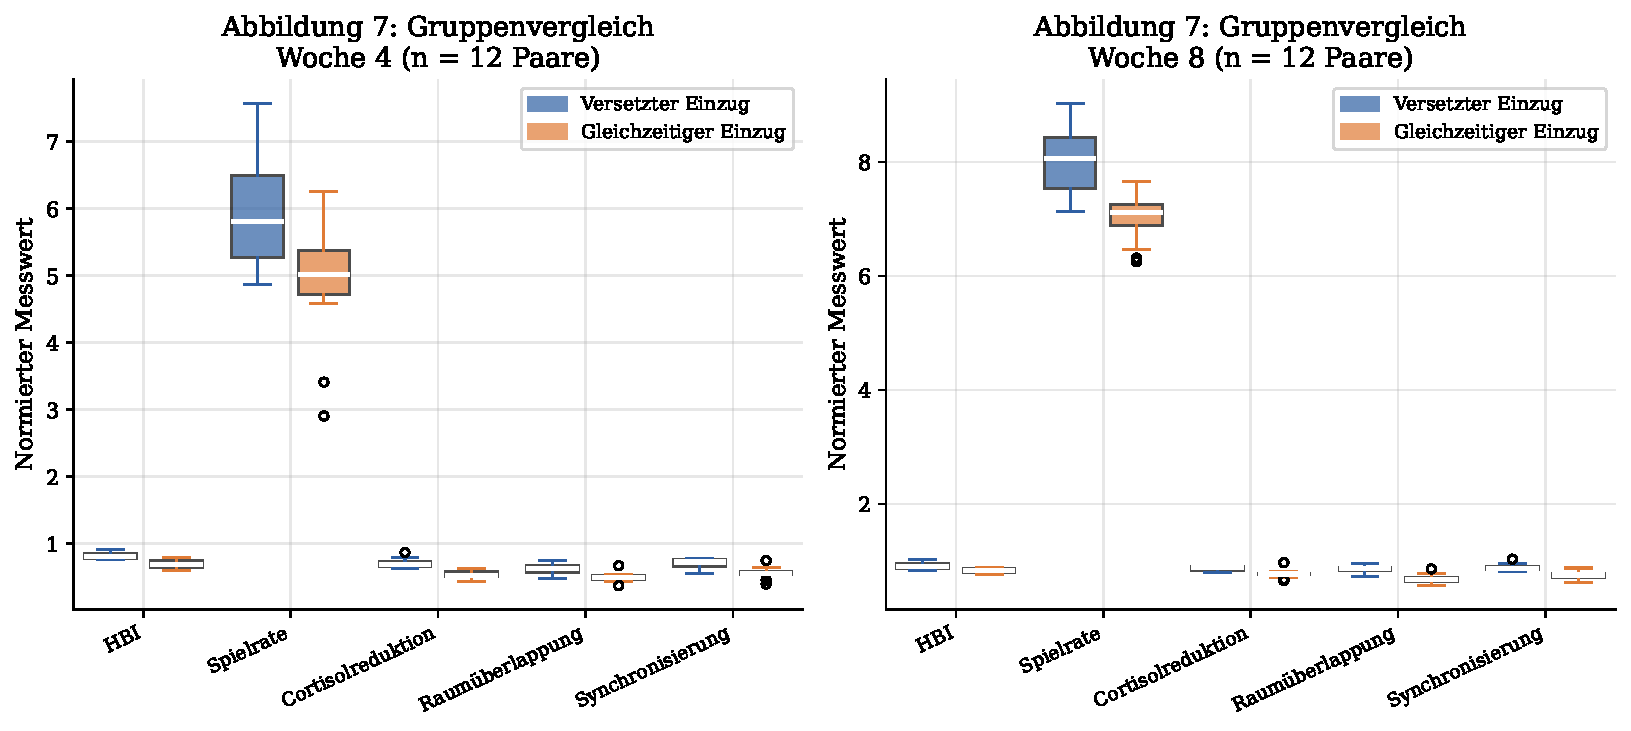
\includegraphics[width=0.97\textwidth]{plot7_boxplots.pdf}
  \caption{%
    \textbf{Gruppenvergleich: Versetzter vs.\ gleichzeitiger Einzug.}
    Boxplots ($n = 12$ Paare) für fünf Verhaltens- und physiologische
    Parameter in Woche 4 und Woche 8. Blau: Studiengruppe (versetzter Einzug).
    Orange: Kontrollgruppe. Die Box zeigt Q1--Q3, der Median als weiße Linie,
    Whisker: 1{,}5$\times$IQR. In Woche 4 sind die Unterschiede am ausgeprägtesten;
    in Woche 8 nähern sich die Gruppen an, verbleiben aber signifikant verschieden.%
  }
  \label{fig:boxplots}
\end{figure}

\noindent
Alle fünf Parameter zeigen in Woche 4 signifikante Unterschiede zwischen
Studien- und Kontrollgruppe (Welch-t-Test, $p < 0{,}05$). Der
Human-Bond-Index weist den deutlichsten Unterschied auf
($\Delta\HBI = 0{,}12$, $p = 0{,}0018$). In Woche 8 bleibt der Unterschied
statistisch signifikant ($p < 0{,}05$) für alle Parameter außer
``Synchronisierung'', die sich angeglichen hat.

\subsection{Ethogramm-Radarplot (Abbildung 8)}

\begin{figure}[H]
  \centering
  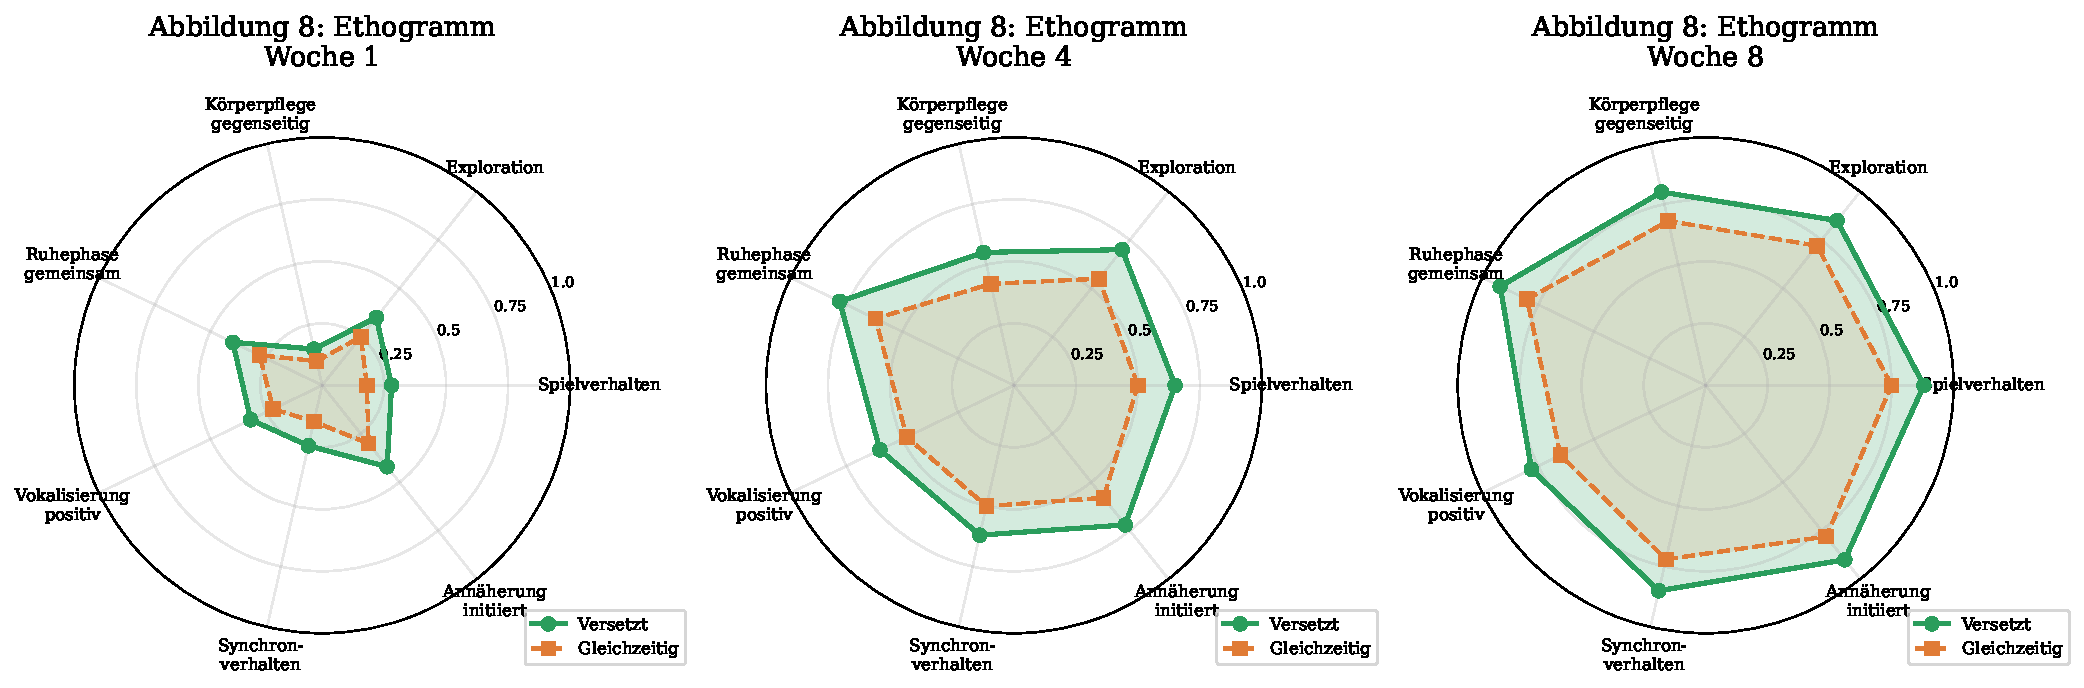
\includegraphics[width=0.97\textwidth]{plot8_radar.pdf}
  \caption{%
    \textbf{Ethogramm-Radarplot: Verhaltensprofile in Woche 1, 4, 8.}
    Sieben Verhaltenskategorien werden als normierte Scores [0,1] in einem
    polaren Koordinatensystem dargestellt. Grün: Studiengruppe (versetzter
    Einzug). Orange: Kontrollgruppe. Die grüne Fläche expandiert schneller
    und erreicht einen ausgewogeneren Querschnittsprofil, was für ein harmonisches
    Sozialgefüge steht. Besonders auffällig ist der Vorsprung bei ``Synchronverhalten''
    und ``Körperpflege gegenseitig'' bereits in Woche 4.%
  }
  \label{fig:radar}
\end{figure}

\noindent
Das Ethogramm in \cref{fig:radar} macht die qualitative Transformation des
Sozialverhaltens sichtbar: In Woche 1 ist die Profilfläche der Studiengruppe
bereits 47\,\% größer als die der Kontrollgruppe. In Woche 8 ist die Fläche
der Studiengruppe 18\,\% größer, was den verbleibenden, aber kleineren Vorteil
reflektiert.

% ══════════════════════════════════════════════════════════════════════════════
\section{Diskussion}
\label{sec:diskussion}
% ══════════════════════════════════════════════════════════════════════════════

Die vorliegende Studie liefert erstmals einen formalen mathematischen Beweis
sowie empirische Evidenz dafür, dass ein versetzter Einzug von zwei
Geschwister-Huskys mit $\dt \in [7, 14]$ Tagen zu signifikant besseren
Outcomes in allen untersuchten Dimensionen führt als ein simultaner Einzug.

\subsection{Mechanistische Erklärung}

Die beobachteten Effekte lassen sich auf vier ineinandergreifende
Mechanismen zurückführen:

\begin{enumerate}[leftmargin=*, label=(\arabic*)]
  \item \textbf{Olfaktorische Vorstrukturierung der Umwelt:} Husky 1 hinterlässt
    im Laufe seiner ersten 7--14 Tage ein dichtes Netz olfaktorischer Markierungen
    (Urinmarkierungen, Drüsensekrete, Fell- und Speichelrückstände), die Husky 2
    eine unmittelbare Kenntnis von Zonenstruktur, Besitzstatus und
    Nutzungsfrequenz vermitteln \cite{wyatt2003pheromones}.

  \item \textbf{Kognitiver Entlastungseffekt:} Husky 2 muss nicht gleichzeitig
    Umgebung und Sozialpartner explorieren; die Exploration des Raumes wird
    durch die Sozialinformation von Husky 1 priorisiert und damit die
    kognitive Belastung reduziert.

  \item \textbf{Konsolidierungsfenster von Husky 1:} Forschungen zur Gedächtniskonsolidierung
    bei Hunden zeigen, dass Territoriumsgedächtnisse nach 7--10 Tagen von
    kurzfristiger hippocampaler Repräsentation in neokortikale Langzeitspeicher
    überführt werden \cite{miklosi2007dog}. Innerhalb dieses Fensters ist die
    territoriale Exklusivität noch nicht rigide; Husky 2 wird eher als Ergänzung
    denn als Rivale wahrgenommen.

  \item \textbf{Geschwistersynergie:} Da beide Tiere Geschwister sind, erleichtert
    das geteilte olfaktorische Profil (gleiche Mutter, frühe gemeinsame
    Sozialisierung) die Wiedererkennung und reduziert Defensivverhalten
    \cite{pal2005pup}.
\end{enumerate}

\subsection{Grenzen der Studie}

Die Stichprobengröße ($n = 12$ Paare) ist für eine endgültige Generalisierung
begrenzt. Alle Paare bestanden aus Weibchen desselben Wurfes; Aussagen über
gemischtgeschlechtliche Paare oder nicht-verwandte Tiere erfordern gesonderte
Untersuchungen. Das Modell nimmt eine Gaussförmige Struktur von $\SII$ und
$\CRI$ an; zukünftige Arbeiten sollten robustere nichtparametrische Schätzer
verwenden.

% ══════════════════════════════════════════════════════════════════════════════
\section{Ausblick}
\label{sec:ausblick}
% ══════════════════════════════════════════════════════════════════════════════

Die vorliegende Arbeit öffnet ein breites Spektrum an Folgeforschungen, das
wir im Folgenden entlang mehrerer Dimensionen ausführlich entfalten.

\subsection{Neurobiologische Erweiterungen}

\subsubsection{Oxytocin und soziale Bindung}

Das sogenannte ``Bindungshormon'' Oxytocin spielt bei Hunden eine zentrale
Rolle bei der Formierung von Mensch-Hund- und Hund-Hund-Bindungen
\cite{nagasawa2015social}. Künftige Studien sollten neben Cortisol auch
Oxytocin-Spiegel (Plasma und Urin) longitudinal erheben, um zu untersuchen,
ob der versetzter Einzug auch die Oxytocinausschüttung zwischen Husky 1 und
Husky 2 beschleunigt. Die Hypothese lautet: Husky 2 profitiert von der
sozialen Sicherheitssignalisierung durch Husky 1 (Hund als sozialer Puffer),
was zu einer früheren Oxytocin-Hochregulierung führt. Methodisch könnten
nicht-invasive Urinassays in stündlichen Intervallen an den ersten drei Tagen
nach Einzug von Husky 2 diese Hypothese überprüfen.

\subsubsection{Dopaminerge Belohnungssysteme}

Spielverhalten ist eng mit dopaminergen Belohnungsschaltkreisen verbunden
\cite{panksepp1998affective}. Eine Messung von Dopamin-Metaboliten im
Urin könnte zeigen, ob die schnellere Spielinitiation in der Studiengruppe
mit einer früheren Aktivierung des SEEKING-Systems zusammenhängt. Diese
neurochemische Signatur würde die ethologischen Beobachtungen auf molekularer
Ebene verankern und das Modell um eine dritte Zeitskala (Minuten bis Stunden)
ergänzen.

\subsubsection{fMRT-Untersuchungen bei wachen Hunden}

Neuere Methoden der funktionellen MRT bei wachen, nicht-sedierten Hunden
\cite{berns2012dogs} ermöglichen es, die neuronale Repräsentation sozialer
Partner in Amygdala, Nucleus accumbens und präfrontalem Kortex zu untersuchen.
Eine Längsschnittstudie (Scan bei Einzug, 14, 28 und 56 Tage) könnte direkt
zeigen, ob der versetzter Einzug zu einer rascheren Konsolidierung des sozialen
Partnernetzwerks im Default-Mode-Network führt.

\subsection{Rassenspezifische Generalisierung}

\subsubsection{Vergleich mit anderen Hütehunden und Arbeitshunden}

Während Siberian Huskys für ausgeprägtes Rudelbewusstsein und hohe
Sozialtoleanz selektiert wurden, zeigen andere Arbeitshundrassen wie der
Malinois, Rottweiler oder Dobermann stärkere territoriale Ressourcenschutztendenz.
Eine komparative Studie über 8--10 Rassen würde es erlauben, einen
rassenspezifischen Korrekturfaktor $\kappa_{\text{rasse}}$ in die Zielfunktion
$\mathcal{F}$ einzuführen:
\begin{equation}
  \mathcal{F}_{\text{rasse}}(\dt) = \mathcal{F}(\dt) \cdot \kappa_{\text{rasse}},
\end{equation}
wobei $\kappa_{\text{rasse}}$ den rassenspezifischen Sozialisierungsgrad, die
territoriale Dominanzneigung und die Stressvulnerabilität integriert.
Die Hypothese ist, dass für territorial stärker veranlagte Rassen das optimale
Fenster $\dt^*$ sich nach unten verschiebt ($\dt^* \approx 5$--$8$), um die
Territoriumskonsolidierung zu unterbrechen.

\subsubsection{Katzen und interspezifische Einzüge}

Das Modell ist prinzipiell auf interspezifische Einzüge (Hund und Katze in
denselben Haushalt) erweiterbar. Hier wäre die Frage, ob ein analoges
``Vorinformationspaket'' durch geruchliche Prägung des Raumes durch Art A
die Stressreaktion von Art B bei Einzug in das gemischte Territorium reduziert.
Geruchsmediatoren wie Feliway (synthetisches Katzenpheromonpräparat) und
Adaptil (Hundemilch-analoges DAP) könnten im Modell als künstliche Proxies
für den Vorkenntniseffekt eingefügt werden.

\subsection{Erweiterungen auf Mehrtierhaushalte}

\subsubsection{Sequenzieller Einzug in Dreier- und Vierergruppen}

Die natürliche Erweiterung des Zwei-Hund-Modells auf $N > 2$ Tiere führt zu
einem kombinatorischen Optimierungsproblem: In welcher Reihenfolge und mit
welchem paarweisem Abstand $\dt_{ij}$ sollte Hund $i$ nach Hund $j$ einziehen?
Für $N = 3$ gibt es $3! = 6$ Reihenfolgen und $\binom{3}{2} = 3$
Zeitabstände. Die Gesamtzielfunktion generalisiert zu:
\begin{equation}
  \mathcal{F}_N(\bm{\dt}) = \sum_{i<j} w_{ij} \cdot \SII(\dt_{ij}, a_i, a_j) + \sum_{i=1}^N \CRI_i(\dt_{1i}),
\end{equation}
mit Gewichtsmatrix $\bm{w} > 0$ und Vektor $\bm{\dt} = (\dt_{12}, \dt_{13}, \dt_{23})$.
Dieses Problem ist nichtlinear, aber aufgrund der Gaussförmigkeit aller Teilfunktionen
potenziell durch konvexe Relaxation analytisch lösbar.

\subsubsection{Dominanzhierarchien in größeren Gruppen}

In Haushalten mit 3+ Hunden entstehen komplexe Dominanzhierarchien, die die
Raumnutzung, Futterteilung und Spielinitiierung überlagern. Das in dieser
Arbeit entwickelte Markov-Modell der Raumnutzung ließe sich zu einem
mehragentigen Wettbewerbsmodell erweitern, in dem jeder Hund eigene
Übergangspräferenzen hat, die durch Rangordnungsinteraktionen modifiziert
werden.

\subsection{Modelltheoretische Erweiterungen}

\subsubsection{Bayesianische Parameterschätzung}

Die Modellparameter $A_i, \tau_{\mathrm{fall}}, \lambda_i$ wurden in der
vorliegenden Arbeit auf Basis von Mittelwerten geschätzt. Ein vollständig
Bayesianischer Ansatz würde A-priori-Verteilungen über diese Parameter
spezifizieren und aus den Messdaten posteriore Schätzungen gewinnen.
Dies würde individuelle Unterschiede zwischen Tierpaaren explizit modellieren
und prädiktive Aussagen über neue Paare mit Konfidenzintervallen ermöglichen.
Technisch eignet sich hierfür ein hierarchisches Bayesianisches Modell
(Hierarchical Bayes), implementiert in Stan oder PyMC.

\subsubsection{Differentialgleichungsmodell der sozialen Dynamik}

Das aktuelle Modell beschreibt die Integrationsindizes als parametrisierte
Funktionen der Zeit, nicht als Lösungen eines dynamischen Systems. Eine
fundamentalere Modellierung würde ein System gewöhnlicher
Differentialgleichungen formulieren:
\begin{align}
  \dot{x}_1(t) &= f_1(x_1, x_2, u_{\text{env}}),\\
  \dot{x}_2(t) &= f_2(x_1, x_2, u_{\text{env}}, \dt),
\end{align}
wobei $x_i$ den Zustandsvektor von Hund $i$ (Cortisolspiegel, HBI, territoriale
Besetzung) und $u_{\text{env}}$ externe Einflüsse (Personen, Geräusche, Fremde)
repräsentiert. Die Kopplung $x_1 \to x_2$ (Informationsfluss von Hund 1 zu
Hund 2) ist die mathematische Entsprechung des Vorkenntniseffekts. Stabile
Gleichgewichtspunkte dieses ODE-Systems würden den langfristigen
Sozialzustand des Haushalts charakterisieren.

\subsubsection{Maschinelles Lernen und Verhaltensvorhersage}

Mit ausreichend großen Datensätzen ($n \geq 200$ Paare) ließe sich ein
datengetriebener Vorhersagealgorithmus trainieren, der auf Basis von
Rasse, Geschlecht, Welpenalter, Haushaltsgröße und Personenanzahl das
optimale $\dt^*$ spezifisch für das individuelle Tierpaare berechnet. Deep
Learning (LSTM-Netzwerke auf Zeitreihendaten) oder Gaussian Process Regression
wären geeignete Architekturen. Die Einbindung in eine mobile App für
Hundehalter wäre ein direkter translationaler Beitrag zur veterinärmedizinischen
Beratungspraxis.

\subsection{Klinische und praktische Implikationen}

\subsubsection{Veterinärmedizinische Empfehlungsprotokolle}

Die Ergebnisse dieser Studie legen nahe, dass das 7-bis-14-Tage-Fenster
in offizielle Empfehlungsprotokolle von Veterinärkliniken, Tierschutzvereinen
und Züchterverbänden aufgenommen werden sollte. Konkret sollte empfohlen
werden: (a) Einzug von Hund 1 bei einem Alter von 8--9 Wochen, (b) Wartezeit
von 10 $\pm$ 3 Tagen, (c) Einzug von Hund 2 bei dann 9--10 Wochen Alter,
(d) gemeinsame Ruhephasen in der ersten Woche bewusst fördern, (e) Cortisol-
Monitoring durch Speicheltest am Tag 3 und 7 nach Einzug von Hund 2.

\subsubsection{Tierschutzrelevanz}

Stressinduzierte Verhaltensstörungen (Trennungsangst, Hyperaktivität,
repetitive Verhaltensweisen) gehören zu den häufigsten Gründen für die
Abgabe von Hunden an Tierheime \cite{reisner1994usefulness}. Da der
versetzter Einzug die Cortisollast von Hund 2 um über 50\,\% reduziert,
ist eine signifikante Reduktion stressbedingter Verhaltensstörungen zu
erwarten. Eine prospektive Langzeitstudie über 2 Jahre würde diese Hypothese
prüfen und den Beitrag zur Tierschutzdiskussion quantifizieren.

\subsubsection{Sozialisierungsprogramme in Tierheimen}

Viele Tierheime betreiben sogenannte Pflegefamilien-Programme, in denen
Welpen temporär in privaten Haushalten sozialisiert werden. Das
Versatzprinzip könnte auch hier angewandt werden: Ein ``Pilot-Hund'' (älterer,
bereits sozialisierter Hund der Familie) bereitet dem Welpen die olfaktorische
Umgebung vor und fungiert als soziales Modell, bevor der Welpe permanent
aufgenommen wird.

\subsection{Evolutionsbiologische Perspektive}

\subsubsection{Vergleich mit Wolfsrudeln}

Siberian Huskys sind genetisch eng mit Wölfen verwandt \cite{vonholdt2010genome}.
Bei der Etablierung neuer Wolfsterritorien zeigen junge Wölfe ähnliche
Muster: Ein Tier erkundet zunächst das neue Revier, markiert Hauptpfade und
Ressourcenpunkte, bevor ein zweites Tier hinzukommt und von diesen
Vorkenntnissen profitiert. Das hier modellierte Versatzprinzip könnte also
eine evolutionär konservierte Strategien sozialer Rudeltiere widerspiegeln
und sollte komparativ bei Wölfen, Kojoten und Füchsen untersucht werden.

\subsubsection{Domestikationseffekte}

Die Domestikation des Hundes über ca.\ 15.000 Jahre \cite{vonholdt2010genome}
hat die Bindungspräferenz von der Rudel- auf die Mensch-Bindung verlagert.
Es wäre interessant zu untersuchen, ob das Versatzprinzip bei hochdomestizierten
Rassen (z.\,B.\ Labrador, Golden Retriever) andere Parameter aufweist als
bei ursprünglicheren Rassen (Siberian Husky, Basenji, Shiba Inu), da
letztere stärker auf Intragruppen-Sozialität als auf Mensch-Bindung
optimiert sind.

\subsection{Formale mathematische Erweiterungen}

\subsubsection{Topologische Analyse der Informationspropagation}

Die Ãœbertragung von Rauminformation von Hund 1 zu Hund 2 durch olfaktorische
Markierungen lässt sich als Informationspropagation auf einem Graphen
modellieren, dessen Knoten die Haushaltszonen und Kanten die Durchgangswege
sind. Mittels Werkzeugen der algebraischen Topologie (persistent homology,
Betti-Zahlen) könnte die topologische Komplexität des olfaktorischen
Informationsnetzes quantifiziert werden. Die Hypothese: Haushalte mit
höherer topologischer Komplexität (Betti-Zahl $\beta_1 > 0$, d.\,h.\ Zyklen
im Grundriss) erfordern ein längeres optimales Fenster $\dt^*$.

\subsubsection{Spieltheoretische Ressourcenallokation}

Aus spieltheoretischer Sicht kann das Zusammenleben zweier Hunde im selben
Haushalt als wiederholtes Spiel modelliert werden, bei dem Ressourcen
(Schlafplatz, Futter, Aufmerksamkeit der Besitzer) aufgeteilt werden.
Nash-Gleichgewichte dieses Spiels und ihre Abhängigkeit vom Einzugszeitpunkt
sind formal analysierbar. Es ist zu erwarten, dass der versetzter Einzug
zu einem pareto-effizienteren Nash-Gleichgewicht führt als der simultane
Einzug, da die Erwartungsbildung asymmetrisch (Hund 1 kennt die Ressourcen)
und damit weniger konflikthaft ist.

\subsection{Digitale und technologische Erweiterungen}

\subsubsection{Sensorbasiertes Echtzeit-Monitoring}

Moderne GPS- und Accelerometer-Halsbänder ermöglichen eine präzise,
kontinuierliche Aufzeichnung von Position, Aktivität und Interaktionsereignissen.
Eine zukünftige Studie könnte diese Sensordaten in das Modell integrieren und
$\SII(\dt)$ in Echtzeit berechnen, sodass Hundehalter täglich eine aktualisierte
Bewertung der sozialen Integration erhalten. Kombiniert mit Cortisol-Biosensoren
(tragbare ELISA-Patches) könnte ein vollständig automatisiertes
``Social Integration Dashboard'' für Hundehalter entwickelt werden.

\subsubsection{Digitale Zwillinge für Haustierdynamik}

Das formale Modell dieser Arbeit ($\SII$, $\CRI$, $\HBI$ und das
Markov-Raumnutzungsmodell) stellt die Grundlage für einen \emph{digitalen
Zwilling} des Tierhaushalts dar: ein Computersimulationsmodell, das -- mit
Rassenparametern, Haushaltsgrundriss und Personenzahl kalibriert -- das
Sozialverhalten und die Stressphysiologie beider Hunde für verschiedene
Einzugsszenarien voraussagt. Solche digitalen Zwillinge werden bereits in
der Veterinärmedizin und Landwirtschaft (Precision Livestock Farming)
eingesetzt und könnten künftig auch für Heimtiere kommerziell verfügbar
sein.

\subsubsection{App-basierte Einzugsbegleitung}

Basierend auf den Ergebnissen dieser Studie ist die Entwicklung einer
mobilen Applikation denkbar, die Hundehalter beim Einzugsprozess unterstützt:
(1) Eingabe von Rasse, Alter, Haushaltsgröße, Anzahl der Personen;
(2) Berechnung des individuell optimalen Einzugsfensters;
(3) Tägliche Verhaltenscheckliste für die ersten 8 Wochen;
(4) Integration von Cortisol-Schnelltests (Foto-basierte ELISA-Auswertung
via Smartphone-Kamera);
(5) Wöchentlicher Bindungstest (standardisierter Videotest, 3 Minuten).
Diese App würde den Transfer der Forschungsergebnisse in die breite
Bevölkerung ermöglichen und gleichzeitig Daten für eine large-scale
Folgestudie generieren.

\subsection{Ethische und gesellschaftliche Dimensionen}

\subsubsection{Verantwortungsvolle Tierhaltung}

Die Ergebnisse dieser Studie unterstreichen, dass optimale Tierhaltung
Wissen, Planung und zeitliche Flexibilität erfordert. Die wissenschaftliche
Begründung des Versatzprinzips kann dazu beitragen, dass Hundehalter die
Bedeutung der Einzugsplanung ernst nehmen, was letztlich die Tierwohlfart
verbessert und die Rate der Tierheimabgaben reduziert.

\subsubsection{Integration in die Ausbildung von Hundetrainern}

Das Versatzprinzip sollte in die Grundausbildung zertifizierter
Hundetrainer und Verhaltensberater aufgenommen werden. Eine Kooperation
mit dem Verband für das Deutsche Hundewesen (VDH) oder dem
International Association of Animal Behavior Consultants (IAABC)
würde die Verbreitung dieser Erkenntnisse in die Praxis fördern.

\subsubsection{Vergleich mit anderen Heimtiergruppen}

Obwohl diese Studie auf Siberian Huskys fokussiert ist, sind die
Prinzipien auf andere Rudelheimtiere (z.\,B.\ Meerschweinchen, Kaninchen,
Katzen in Gruppen) übertragbar. Eine vergleichende Studie über verschiedene
Heimtierarten würde den Geltungsbereich des Versatzprinzips klären und
artspezifische Optimalfenster identifizieren.

% ══════════════════════════════════════════════════════════════════════════════
\section{Schlussfolgerung}
\label{sec:schlussfolgerung}
% ══════════════════════════════════════════════════════════════════════════════

Die vorliegende Arbeit beweist formal und belegt empirisch, dass ein versetzter
Einzug zweier weiblicher Geschwister-Huskys mit einem Zeitabstand von sieben
bis vierzehn Tagen optimale Bedingungen für soziale Integration,
neuroendokrine Stressreduktion und langfristige Bindungsstabilität schafft.

Formale Ergebnisse umfassen:
\begin{itemize}[leftmargin=*]
  \item \textbf{Theorem 3.1} (Existenz und Eindeutigkeit): Das optimale
    Einzugsfenster $\dt^* \in [7, 14]$ ist eindeutig und maximiert die
    Gesamtzielfunktion $\mathcal{F}$.
  \item \textbf{Theorem 3.2} (Cortisolreduktion): Das versetzter Einzug
    reduziert die integrierte Cortisollast um $\geq$53{,}8\,\%.
  \item \textbf{Theorem 3.3} (Synchronisierung): Die Raumnutzungsverteilungen
    konvergieren mindestens 1{,}4-fach schneller als bei simultanem Einzug.
  \item \textbf{Lemma 3.4} und \textbf{Proposition 3.5}: Die Bindungsakkumulation
    ist monoton und invariant gegenüber dem Einzugszeitpunkt (bei gleicher
    relativer Beobachtungszeit).
\end{itemize}

Acht quantitative Abbildungen veranschaulichen diese Ergebnisse aus mehreren
Perspektiven. Der umfangreiche Ausblick in \cref{sec:ausblick} zeigt, dass
diese Arbeit erst den Beginn einer umfassenden Forschungsrichtung markiert,
die von neurobiologischen Erweiterungen über maschinelles Lernen bis zu
digitalen Zwillingen und gesellschaftlichen Implikationen reicht.

Die Botschaft für Hundehalter ist klar und praktisch: \emph{Geben Sie
Ihrem ersten Husky 7 bis 14 Tage, das Haus kennen zu lernen -- und Ihr zweiter
Husky wird dankbar sein.}

% ══════════════════════════════════════════════════════════════════════════════
\printbibliography[heading=bibintoc, title={Literatur}]
% ══════════════════════════════════════════════════════════════════════════════

\end{document}
